\chapter{Simulation Optimisation with Aspect Orientation}
\label{chap:exp1_simulation_optimisation}
\label{chap:experiment_setup}

\inline{
  My main concern with this chapter at time of writing (10-10-23) is that it
  goes into too much trivial detail (e.g. types passed into different
  functions), and not enough into substantive detail (experimental design and
  why things are set up the way they are). Maybe I have enough substantive
  detail, but just a surplus of trivial detail? Consider this carefully when
  redrafting and kill your darlings. If you're not Tom and you're reviewing
  this, please be generous in suggesting things to eliminate!
}

\inline{
  Another thought on the issues with this chapter. There are currently two
  ``Experimental Design'' chapters. The second is trying to lay out how we'll
  build statistical measurements etc around the model \& advice described
  earlier; the first is giving an overview of the experiment and what'll happen.
  I think both are ambiguously titled and should both be renamed. However, an
  ``Aims'' section also exists before the first ``Experimental Design'' section,
  and I think this is a sign I'm waffling a \emph{lot} and not getting to the
  point. Needs to be reviewed and cut down significantly.
}

\inline{
  ANOTHER observation on this ``aims'' section. I need to properly explain the
  experimental design early on, and I don't make any reference at all to the
  prior distribution model at the moment. I think the aims section should
  contain almost exclusively an explanation of the experimental design. Right
  now it's a combination of experimental design and justifying using pdsf... which
  I can probably do in 2 sentences instead of a page and a half.
}

This chapter describes the design and implementation experiments which
investigate the use of advice to augment behaviour in a model. The experiments'
foundation is RPGLite, described in \cref{chap:rpglite}, which was deployed and
played on iOS and Android~\cite{RPGLiteLessonsLearned}. Data collected about
players' interactions with the game can be used to simulate individual players'
behaviours. Data produced by simulated RPGLite play can also be compared against
the real-world dataset to assess whether a simulation is accurate. This chapter
describes the design and implementation of experiments which use this
opportunity to investigate whether \aop{} can augment behaviour in a model.
%These experiments answer several research questions:

%\begin{itemize}
%  \item \rqtwo{}
%  \item \rqthree{}
%  \item \rqfour{}
%\end{itemize}

Each experiment applies advice to a model of RPGLite play to evaluate a research
question. The experiments share a significant proportion of their design and
implementation. As their common elements require a significant amount of
explanation, a chapter outlining both the setup \emph{and} results of these
experiments would be extremely long, and their shared foundation means that they
are most naturally explained together. For this reason, the design and
implementation of \emph{all} experiments is explained in this chapter, and their
results follow in \cref{chap:experimental_results}.

The common aspects of design and implementation in this chapter are explored as
follows. \inline{After completing the restructuring of these chapters, come back
and complete this chapter outline.}



\section{Aims}\label{sec:aop_simulation_optimisation_aims}

\inline{
  I think this ``Aims'' section is waffly and possibly unneccessary but I
  haven't copy-edited it yet. REVISIT.
}

Previous simulation and modelling efforts using \aop{} have focused on
using aspects to compose model or simulation details\inline{There must be
tons of good citations for aspects being used to compose together a simulation /
model}\revnote{We don't think this is the case --- those citations just don't
exist! Rework to discuss use of AOP in business process modelling, and note that
nobody made those models in practice, just tooling.}\revnote{Also, just read
this and noted that while AOP isn't necessarily used for model composition,
there \emph{are} lots of projects for modelling via composition, just not using
AOP. Although perhaps I can just cite tooling here, and ancillary projects like
aspect-oriented lindenmeyer systems\ldots{}?}. Critics of aspect orientation
note that the act of oblivious process composition makes understanding codebases
difficult, and so ensuring that a simulation properly models real-world
behaviour is made trickier with the introduction of aspect orientation.
\inline{this last sentence doesn't make much sense to me when reviewing.}
However, aspect orientation might instead be used to \emph{augment} an existing
model, by rethinking what aspects are used to represent.

An alternative use of aspects would be to first build a non-aspect-oriented
model of \emph{expected} behaviour, and separately build aspects which describe
deviations from this. For example, one might more realistically simulate safety
procedures by first producing an idealised, ``naive'' model of what employees
are expected to do, and separately model alterations to prescribed behaviour as
an employee's boredom, expectation that checks and balances are unnecessary
wastes of their time, and so on --- effectively, separating out models of
degraded modes~\cite{johnson2007degradedmodes}.

Previous research on the use of aspect orientation to model degraded modes
adopted the traditionally claimed benefit of aspect orientation: separation of
cross-cutting concerns, allowing for a greater reusability of
codebases~\cite{wallis2018caise}. A repository of cross-cutting concerns in
socio-technical simulation such as boredom was developed as a library to be
applied to any future models~\cite{fuzzimoss_repo}. However, aspects used in
simulation have no intrinsic need to represent concerns that are cross-cutting.
Indeed, whether they can be accurately used to represent cross-cutting concerns
in simulation is the topic addressed in \inline{Add a cross-reference to the
chapter on cross-cutting concern simulation accuracy when it exists}. Aspects
might instead be used to represent \emph{amendments to processes} which deviate
from an expected norm, in this case represented by the idealised model aspects
are applied to.

To more concretely relate this to the experiment at hand: play of RPGLite can be
modelled as players matchmaking, picking characters, and then mutually taking
turns until one player's characters are entirely expired. Once a player's
characters are dead, new matches can be made. This can continue indefinitely.
Lacking a heuristic to select next moves or characters, players might be
modelled as picking random moves. However, heuristics for move selection can be
added to the naive model of play by way of augmenting the processes already
defined through aspects. This approach can be useful both when
modelling player behaviour generally and when modelling the behaviour of
individual players: \revnote{Consider making these a para instead of an
enumerated list.}

\begin{enumerate}
    \item Different players might use their own unique heuristics to model play.
    Each player's behaviour is therefore well described by separating what play
    ``looks like'' to what makes a given player play differently to their peers.
    \item Different players might lean more heavily on different heuristics, or
    mixes thereof. Play might be characterised by reliance on experience, on
    recent games, on knowledge of an opponent, and so on; these different
    variables can be expected to be weighted differently by each player, adding
    complexity to the code which models this individualised play.
    \item A modeller might discover a new idea for a heuristic long after
    developing an original concept for a model. Due
    to the impact of \pointno{2}, ideal architectures for an approach such as
    this should allow these heuristics to be defined entirely separately to
    the base model to maximise flexibility when maintaining experiments.
\end{enumerate}

Considering \pointno{1}, \pointno{2}, and \pointno{3}, architectures and
paradigms which enable separation of concerns are well-suited to defining
alternative approaches to play. Some architectural approaches such as mixins or
plugin design patterns might support this structure well, but they typically
rely on language features (in the case of mixins) or knowledge of software
engineering (in the case of design patterns). Aspect orientation is typically
provided to developers as a framework or runtime in a language (such as
AspectJ\cite{aspectj_intro} or PROSE\cite{popovici2002PROSE}) and can require
minimal architectural understanding to use: concepts are simple, and the effort
of composition is alleviated by the supporting framework or runtime.

The approach makes little use of aspect orientation's focus on cross-cutting
concerns, as whether behaviour cross-cuts different parts of a codebase is not
of interest in this use case. Instead, aspect orientation is treated as a
composition mechanism which introduces no additional requirement of technical
knowledge.

\subsection{PyDySoFu Suitability}\label{subsec:optimisation_with_aspects_usingpdsf}
Some aspect orientation frameworks do not adequately achieve this requirement.
For example, the most influential framework, AspectJ, requires the use of
language extensions to define integrate aspect
orientation\cite{AspectJLanguageAndTools}, and similar additional complexity is
added in seemingly every alternative framework, through the use of bespoke
virtual machines, compilers, translators, or
languages\cite{rajan2006nu_towardsAO_invocation,popovici2003JITaspects,AspectCplusplusDesignImpl,baker2002maya}.

PyDySoFu, however, requires very little additional knowledge to use. Its design
prioritises simplicity and a shallow learning curve that makes its adoption by
researchers without a software engineering background feasible: \inline{maybe
cut this list of reasons PyDySoFu is fantastic...}

\begin{itemize}
    \item PyDySoFu is implemented as a pure-python library, meaning that it can
    be installed through Python's package manager (pip) and imported like any
    other Python library. No additional supporting infrastructure is required.
    \item Aspects in PyDySoFu are simple functions which take as arguments
    whichever pieces of information are pertinent for the function's use as an
    aspect\footnote{For example, an ``encore'' aspect which is woven after a
    target procedure returns will be provided that target's return value.}.
    \item To weave a PyDySoFu aspect requires only a method call, which returns a
    \lstinline{callable} which unweaves that aspect.
    \item Defining PyDySoFu pointcuts requires only a regular expression
    matching a method name. This can apply to a wide range of join points if
    required, but where method names are provided directly, the join point is
    made clear.
    \item Additional clarity over where aspects \emph{can} be woven is
    introduced by PyDySoFu's transparent weaving of aspect hooks, mitigating
    some of aspect orientation's most prominent criticisms.
\end{itemize}

PyDySoFu therefore satisfies the requirements of this work well: it offers
composition of procedures outside of the scope of an original codebase, makes
what is being composed where clear to a programmer, and makes no
changes to Python as a language (thereby requiring users to specialise in fewer
tools). 


\subsection{Proposed Experiment}\label{subsec:optimisation_with_aspects_experiment}

Aspect orientation's use as a composition tool for model components makes sense
in principle, but it is unclear whether the addition of behaviours to a naive
model would make the model more ``realistic''. Furthermore, changes to a model
could alter its representation so as to weaken its mimicry of the system it
simulates; adding behaviours could make it \emph{less} realistic. The
fundamental issue at play is that it is unclear whether the changes made would
properly represent what might be empirically observed. While PyDySoFu's design
makes understanding what is being composed simpler than other aspect orientation
frameworks, a composed model under this paradigm is still split across multiple
areas of a codebase, making a visual assessment of whether a model accurately
reflects the intended behaviour impractical. It is therefore important to
demonstrate the efficacy of PyDySoFu and the modelling paradigm it introduces,
by confirming the realism of a model to which behavioural variation is applied.

We can confirm whether aspects can realistically represent changes to a naive
understanding of the real world by comparing their output against empirical
data. For example, if a such a model of behaviour in a system outputs data which
correlates poorly against empirically collected data, a change to that system
would make it more realistic if it improved this correlation, and could be said
to be realistic if the generated data appeared sufficiently ``close'' to the
empirical dataset --- which here means that the correlation between the two is
of statistical significance. Such a change can be aspect-oriented. Therefore, we
can see the application of aspects as the application of packages of potential
improvements to a base model, which can be verified by way of comparison to
known-good datasets.

This is the basis of the experiments in this thesis.

With datasets collected empirically on RPGLite's play, we can build a naive
model of play and aspects to apply that should realistically model data from
players. This can be used to answer the research questions motivated in
\cref{subsec:rqs}\inline{THESE RESEARCH QUESTIONS HAVE BEEN AMENDED SINCE I
  FIRST WROTE THIS SECTION (I hadn't decided on a wording then) AND THE
  PLACEHOLDER SUGGESTION THAT PREVIOUSLY EXISTED WAS JUST WHETHER ASPECTUALLY
  AUGMENTED MODELS COULD BE REALISTIC. THIS CHAP DOES MORE, SO THIS SECTION
  NEEDS TO BE REWORKED.}:

\begin{researchquestion}
  \begin{enumerate}
    \item Can changes to a model be represented as advice using aspect orientation?
    \item Can a model be made more realistic by applying aspect-oriented improvements?
    \item Can advice which improves the realism of a model be ported to others without loss of realism?
  \end{enumerate}
\end{researchquestion}

% To answer this question, a naive model of play is produced, and aspects
% developed which encapsulate different play styles so as to compare empirically
% sourced datasets against both its aspect-augmented and unaltered counterparts.
% The following subsections detail the naive model developed and aspects applied
% to this model.

To answer these questions, a naive model of play is produced. Aspects are
developed which model learning within the system defined by the naive system.
The synthetic datasets produced by models with naive or aspect-applied models
can be compared to an empirical dataset sourced from real-world players of the
game, and their similarity compared.\inline{Rework to include details on the
  other RQs, too .}

``Naive'' is used here to describe a model which does not encode any
understanding of the players of the game being modelled. Traits such as
learning, distraction, or aptitude for similar games are irrelevant to the naive
model. We need a naive model to demonstrate the effectiveness of an
aspect-oriented alternative: we can measure how closely it reflects empirical
data, and compare this against the same measurement drawn from another model
with behavioural variations encoded using aspects. A closer match from our
aspect-oriented model would demonstrate that the technique can enhance a model's
realism. Our naive model also provides a null hypothesis: if no improved
similarity is observed, the technique brought no improvement to the model's
realism. No measurable difference indicates that weaving behavioural variations
as aspects has no impact on a model's realism.

\inline{Write a little here on the learning aspects.}

\inline{Flesh this out as a brief wrap-up of our experimental technique. The end
of our ``naive'' model explanation might be useful to move down here / rework
into this para.} Contrasting the similarity of the empirical dataset to both
naive and aspect-applied datasets\ldots{} This discussion is provided so as to
provide context for the following sections; experimental design is discussed in
more depth in \cref{sec:optimisation_with_aspects_experimental_design}. 


\section{Naive Model}\label{sec:optimisation_with_aspects_naivemodel}

A naive model of play was developed by separating each stage of the actions
taken by players and separating them into individual procedures. The model was
written as a workflow in Python, and state of workflow execution was separated
into three components: the actor that a function invocation (or ``step'')
represents activity from; a ``context'' in the parlance of languages like
Golang, representing the state of a game being played; and the environment in
which that game is played.\footnote{Incidentally, this structure allowed a
flexible and natural implementation of a procedural simulation containing
concepts common in software engineering (such as contexts) and environments
(found in simulation frameworks). We imagine that it is easily adopted in
existing simulation frameworks such as SimPy\cite{simpy_intro}. Some additional
detail is included in \cref{appendix_ace_pattern}.} The naive model of RPGLite
follows a simple workflow mimicking player interaction with the mobile game
deployed. A graphical representation is provided in \cref{fig:naive_model}.
\Cref{fig:naive_model_with_experimental_apparatus} contains a diagram showing
how the naive model is used to produce synthetic data by simulating repeated
gameplay.

\begin{figure}[h]
  \centering
  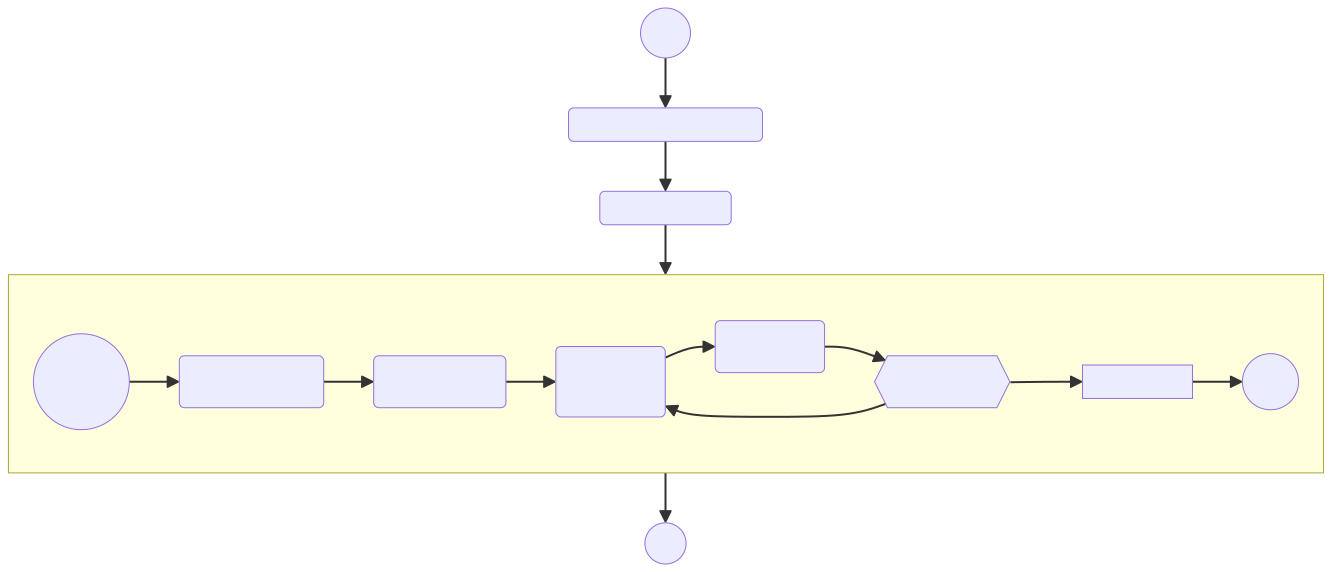
\includegraphics[width=\columnwidth]{60_optimisation_with_aspects/diagrams/naive_model.png}
  \caption{A diagram of the ``naive model'' of RPGLite play used in experiments.}
  \label{fig:naive_model}

  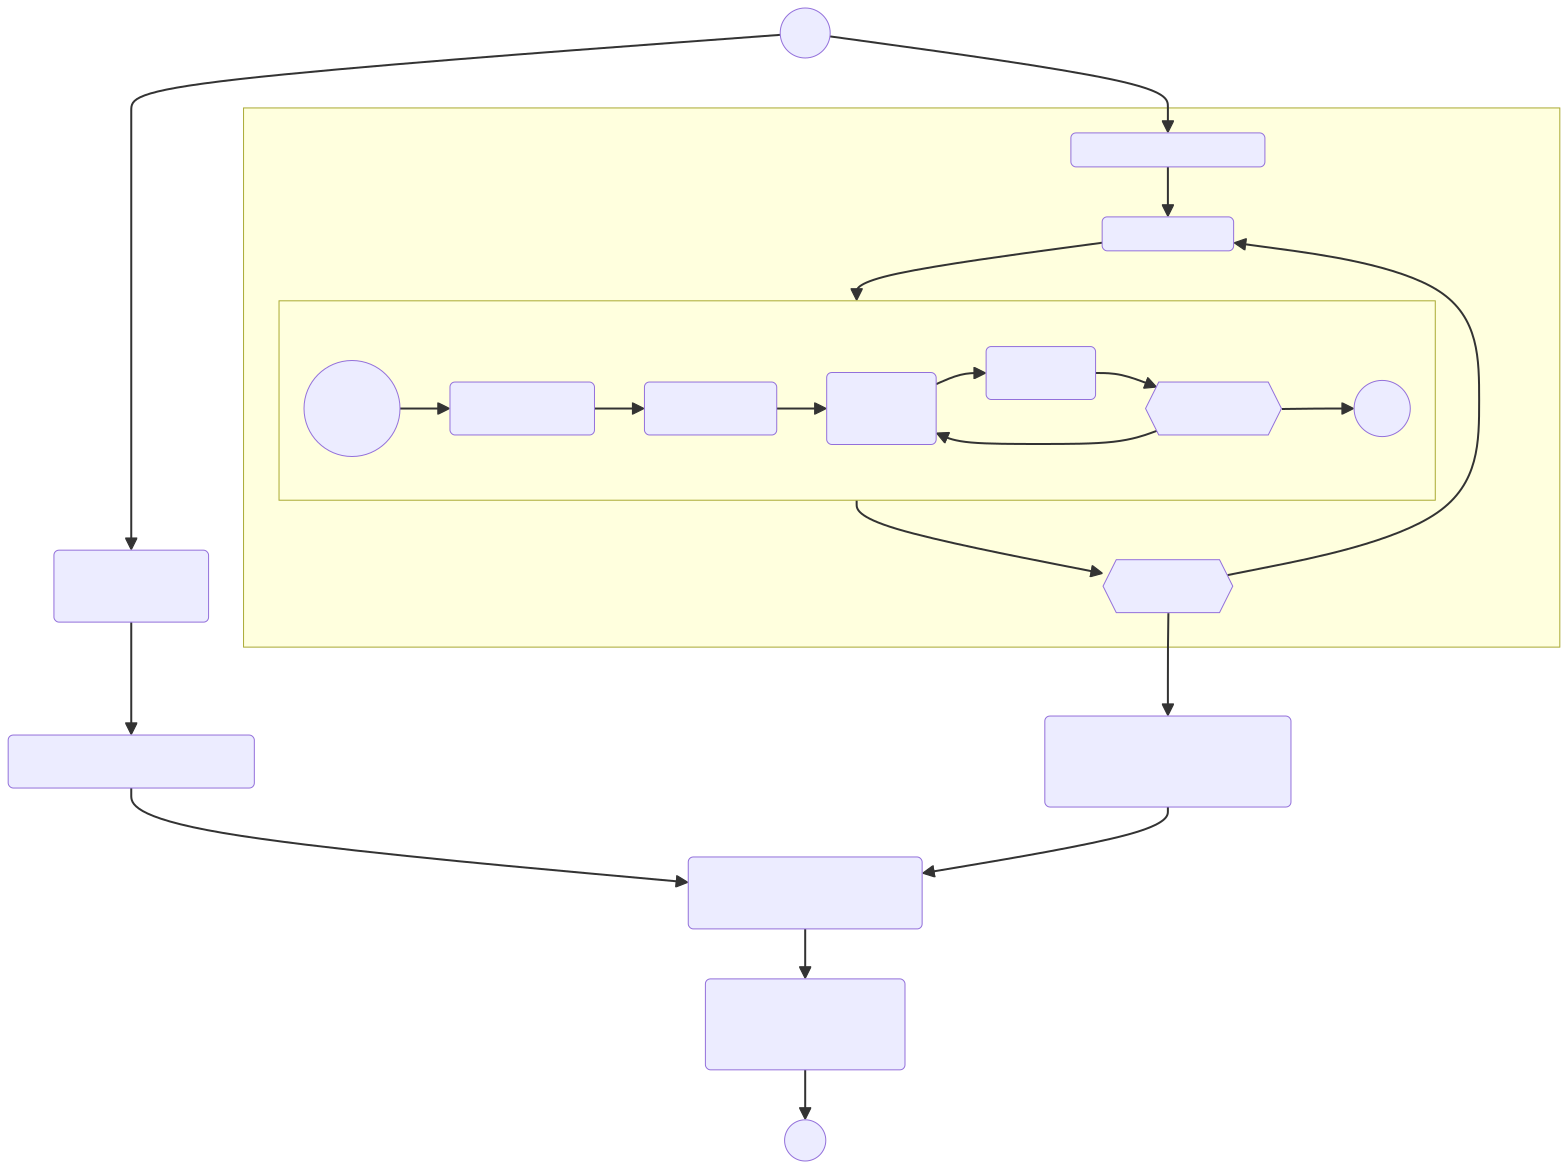
\includegraphics[width=\columnwidth]{60_optimisation_with_aspects/diagrams/experiment_setup_for_datagen.png}
  \caption{A diagram illustrating how the naive model is used to generate datasets used in experiments.}
  \label{fig:naive_model_with_experimental_apparatus}
\end{figure}


\inline{Move mermaid-based figures to .svg for fidelity}

Two randomly-selected players repeatedly select characters to play from the pool
of 8 characters described in \cref{chap:rpglite}, and a player is chosen to play
first at random, referred to as the ``active'' player. That player selects a
random valid move to make. The active player alternates, and the process
repeats, until such time as an active player starts their turn with both of
their characters fully depleted of health. The player with remaining characters
is the victor. When used to generate datasets for analysis, another game is
started by picking another pair of random players and starting a game between
them; this continues until a predetermined number of games has been played.
After a sufficient number of games are played, analysis of the generated datasets
is performed. \footnote{Dataset analysis is explained in
\cref{sec:optimisation_with_aspects_experimental_design}.}
Decisions made by players in the model are random; this is because the model is
designed to avoid informed decisions where possible. This model illustrates the
steps taken by players and disregards whether the simulated players' choices
reflect realistic ones. Informed decisions are woven as \aspectoriented{}
changes to behaviour.





\section{Modelling Learning}\label{learning_model_definition}

The naive model makes choices randomly. Informed decisions are made by weaving
advice into the model which changes player behaviour. Experiments are evaluated
through the distribution of character pairs found in gameplay data, so aspects
are required which change that distribution of character pairs. To change the
distribution of character pairs chosen, an \aspectoriented{} model of learning
is created which alters player behaviour to select character pairs at the
beginning of a game by inferring strong characters from those observed to win
games previously. This section describes its design.

\subsection{What Players Learn}

Players learn many things when playing a game. Other than learning about
characters and their strengths and weaknesses, players also learn how to take
successful turns by making moves strategically. Character pair selection is the
focus of these experiments because they are simpler and have a smaller state
space for players to understand: the ``metagame'' for character pair selections
is the simpler of the two.

\label{metagame_explanation}
A metagame is a community's perception of ``good'' gameplay at a given point in
time. For example, if certain characters are popular, players may select other
characters which are not likely to win against \emph{most} characters but are
likely to win against \emph{currently popular} ones. As a result, players may
select weak characters strategically, and strategically selected characters
change over time in response to changing popular choices in the community.
Similar reasoning applies to move selection. For a more thorough discussion of
the concept of a metagame, see the survey of literature and definitions by
\citet{metagaming_in_esports} or the original but more theoretical work on the
topic by \cref{howard1971metagames_seminal}.

A design consideration of RPGLite is that its metagame is ``solvable'', meaning
that there exists an objectively optimal choice for a player to make in any
state~\cite{kavanagh2021thesis}. As the space of possible moves is much larger
than the space of possible character pair choices players are expected to learn
optimal choices more quickly, which would lead to an unchanging (``stable'')
metagame. In practice, the character selection metagame converged on optimal
character selections, whereas players consistently made errors when selecting
optimal moves~\cite{kavanagh2021gameplay}. As players' choices of character
pairs is therefore easier to model (and more consistent between players), a
model of learning is applied to their character pair selections instead of their
move selections. Player behaviour is altered to select objectively optimal moves
in every state instead of this being learned over time; this is described in
\cref{aspect_to_ensure_best_move}.



\subsection{Literature regarding Learning}
\label{subsec:models_of_learning_discussed}

Different people learn in different ways. Indeed, no universally-accepted
definition of learning appears to exist. This is presumably because it is
convenient to define what it means to learn differently in the context of
different pieces of work. For example, cognitive models of learning can be
useful when considering mental processes specifically, whereas functional models
of learning lend a more empirically applicable perspective. What it means to
learn is outwith the scope of this research; however, the experiments presented
in \cref{chap:experimental_results} include a model of learning. To justify our
model, we consider a functional approach to learning, as this is more closely
linked to the empirically focused work of simulating real-world behaviour than
cognitive alternatives.

\citet{lachman1997learning} summarises standard definitions of learning as
``\textelp{} a relatively permanent change in behavior as a result of practice
or experience''. They observe that these definitions have practical shortcomings
such as a focus on behavioural change (as learning may not change behaviour) or
conflating learning's process and its product (the process by which we learn is
not obviously identical to its result, of which behavioural change is an
example). They suggest learning might be better defined as:

\begin{displayquote}
\textelp{} the process by which a relatively stable modification in
stimulus-response relations is developed as a consequence of functional
environmental interaction via the senses [\ldots{}] rather than as a consequence
of mere biological growth and development~\cite{lachman1997learning}.
\end{displayquote}

They note that their definition distinguishes learning from phenomena such as
injury, changes to one's maturity, or sensory adaptation, incorporates
stimulus-response relationships the research community consider as learned, and
differentiates learning's process and product. Their model is inherently
functional, making it useful for the purposes of simulation and modelling,
although they offer only a definition of learning and a brief comparison to
the standard textbook definition they introduce. The work presented is not
intended to demonstrate its improved model of learning empirically, only to
discuss its semantic merit. However, the models proposed in this thesis require
only a theoretically informed, sound basis for their model of learning, and a
lack of empirical justification is not a barrier to the relevance of the model
\citeauthor{lachman1997learning} proposes.

\citet{de2013learning} propose a functional definition of learning which is
primarily concerned with providing a definition of learning which is both
accurate and useful for the purposes of cognitive learning research. Doing so
attempts to provide a model around which some consensus can be reached; learning
is a central concept in psychology, and they describe their definition as
supportive of cognitive work without requiring a cognitive model. They introduce
their definition as:

\begin{displayquote}
Our definition consists of three components: (1) changes in the behavior of the
organism, (2) a regularity in the environment of the organism, and (3) a causal
relation between the regularity in the environment and the changes in behavior
of the organism.
\end{displayquote}

This model of learning contains more nuance than the ``textbook definitions'' of
learning they paraphrase as ``a change in behaviour that is due to experience''
but does not stray far from the core concept of an environmental stimulus
impacting behaviour in a causal fashion. The introduction of ``regularity'' to
their definition refers to the presence of the stimulus with some form of
repetition, either through multiple instances of a stimulus at different times
or the same stimulus occurring concurrently. \citet{de2013learning} observe that
their model is straightforward without the sweeping inclusivity of the simple
model mentioned earlier and is easily verified (although, as in the work of
\citet{lachman1997learning}, empirical verification is omitted in favour of
semantic analysis).

Aside from other benefits more particular to their research community, these
benefits are especially useful from the perspective of modelling learning in the
case of RPGLite. A simple functional definition can be captured in a software
model and introduces fewer opportunities for misunderstanding or misapplication
than a more complex or theoretical model. It also introduces  concepts such as
regularity and causality other definitions do not. We therefore adopt this
definition as a basis for our model of learning.



\subsection{Modelling Learning Character Pair Selection in RPGLite}
\label{subsec:defining_our_models_of_learning}
\label{learning_model_details}

\revnote{This describes the design of the learning model and it's \emph{pretty
lengthy} --- it's edited to at least make sense, but it could be shorter
if I had the time to rework it entirely.}

We use \citet{de2013learning}'s definition to define an \aspectoriented{} model
of learning that can be applied to the naive model of RPGLite. Their definition
of learning gives criteria that this model must meet: players' behaviour must be
influenced by their learning to meet the definition's first criterion; repeated
experiences in successive games must influence the direction of players'
learning is required by the second; and the third criterion requires that this
must happen in a causal manner. To meet these, the learning model's design
should model a causal relationship between a player's observation of successful
character pairs and their future choices of character pairs.

To fulfil these requirements, a model might draw on previously successful
character pairs to determine future ones. One approach is to model learning as
consistently playing the character pair which most \emph{recently} was observed
to win a game. A completed game must have a winning pair,\footnote{Or be
forfeited, in which case the previously winning pair could be substituted.} and
we can select this pair when playing future games until a different pair is
observed to win instead. However, this does not align with one's intuition of
how players \emph{would} engage with a game in the real world. A player seems
unlikely to be deterred from a strategy they believe is ideal when RPGLite's
random nature gives them an outcome they could percieve as unlucky. We can
expect players to understand that \emph{perfect} play might not be
\emph{winning} play: in some games, the right moves might not lead to a
successful outcome due to moves randomly missing opponent characters. Equally,
players may take time to become confident in a strategy. We would expect a
player to explore character choices before settling on a preferred pair early in
their experience, and would expect experienced players to choose characters
based on what they have learned through their experience rather
than continuing to explore their options. From these observations, we can see that:

\begin{enumerate}
  \item There are scenarios where players can be expected to observe wins/losses
  \emph{without} incurring behavioural change.
  \item Players' confidence in what they have learned can affect their
  inclination to rely on that knowledge when making decisions.
  \item What players learn in successive games would have a small impact in
  their early experiences, but an increasingly significant impact proportional
  to their experience in the game.
\end{enumerate}

The model of learning used to simulate RPGLite players can be explained
following a similar structure: \pointno{1} implies that players' observations
regarding winning characters is separate from behaviour change; \pointno{2} implies
some mechanism determining players' inclination to use their knowledge when choosing
characters (rather than exploring their options); and \pointno{3} implies that
their inclination to rely on their knowledge instead of exploring the state
space is proportional to the amount of experience players have.

To fulfil requirement \pointno{1} and separate win/loss observation from
behaviour change, a player's assessment of how likely a character pair is to win
a game is represented as a probability mass function (\emph{``PMF''}) updated
through its own aspect (which is described in more detail in
\cref{aspects_applied_section}). The PMF maps character pairs to their chance of
being selected by a player, and initially tracks all character pairs as having
an equal chance of being selected. After every game, the chance of selecting the
winning character pair increases, and the chance of selecting any other pair
decreases. The sum of probabilities of being selected across all character pairs
always sums to 1 (100\%). This is implemented as a record of the winning
character pairs observed by a player: many ways of producing a PMF from a
sequence of wins exist, but for the purposes of explanation, one such method is
to take the proportion of wins for every character pair as their probability of
being selected. This method produces a valid PMF because the sum of those
proportions accounts for 100\% of observed wins and losses, so the sum of all
probabilities must also be 100\%.

Requirements \pointno{2} and \pointno{3} are fulfilled through a separate
mechanism to control whether players use this PMF to make decisions. Players are
expected to explore possible options early in their experience, and rely on
their observations when they have completed many games. This is because
\citet{lachman1997learning} identifies that the experience of a learning agent
draws from ``regularity'' in their environment, and requiring many games to be
played before players' behaviour changes ensures that a regular experience is
present.\footnote{Note that the regular experience might be one of the character
pair choice not having an impact at all; if the player observes all character
pairs winning an equal number of times, the PMF would reflect this and player
behaviour would effectively remain random. However, the player would choose each
character pair at an equal rate because they would have learned that the choice
was inconsequential, so even in this scenario learning occurs.} The mechanism
controlling whether players will make decisions based on previous experiences is
referred to as ``confidence'', referring to their confidence in their experiences at a
point in time. A model of confidence fulfils requirement \pointno{2}, and
\pointno{3} is fulfilled by confidence increasing proportionally to players'
experience.


Confidence is modelled in these experiments as a monotonically increasing
function mapping experience (quantified as games played) to confidence as
a percentage chance 0\% and 100\% that a player determines their
character choice based on their observations of wins and losses rather than
exploring the space of possible choices. Players are ``confident'' when making a
decision with the probability determined by their confidence model.

If the player is not confident, their behaviour is unchanged and they select
character pairs randomly as in the naive model. If they are confident, their
behaviour is instead informed by their experiences and they select a character
pair from the distribution defined by the PMF that their historical observations
define. As the PMF affords higher probabilities to repeatedly winning character
pairs, player behaviour is causally affected by the regularity of their
experience. This implements a realistic model of learning in fulfiling the
requirements of the functional model proposed by \citet{lachman1997learning}.

\subsection{Modelling Player Confidence}\label{subsec:confidence_model}

To model confidence we require a function mapping the number of games a player
has completed to a probability between 0 and 1, fitting the crieteria described
in \cref{subsec:defining_our_models_of_learning}. A sigmoid curve fulfils these
requirements: it rises monotonically and produces values between $0$ and $1$. It
also notionally conforms to an intuition around ``confidence'' as a behavioural
trait: like a sigmoid, peoples' confidence starts low and remains so until it
reaches some inflection point, after which one's confidence increases more
signficantly, with the rate of this increase tapering as experience continues to
increase. However, not all real-world players might express the same traits in
their growth of confidence, and this intuition is not universally applicable;
the shape of a players' confidence sigmoids differ in the real world. To answer
the proposed research questions, an ideal model of confidence is not required,
but one which reflects \emph{some} real-world players \emph{is}. To account
for this, the confidence model uses a sigmoid is which can be parameterised to
alter its shape.

A sigmoid curve is suitable for modelling confidence where other curves are not,
because we require a period where players lack confidence and explore their
options. Sigmoid curves such as the logistic~\cite{verhulst1845loi} or
Gompertz~\cite{gompertz1815curve} are widely used when modelling
systems~\cite{werker1997modelling}, but while they fulfil the role of a
monotonically increasing curve with asymptotically low and high initial and
final states, the shape of such curves is not trivially modified to fit
different players' learning styles. To fulfil the confidence model's
requirements it is necessary to find an alternative: different players are
expected to exhibit more bullish or timid styles of play, so the curve should be
parameterised to account for the behaviours of those individuals.

More flexible asymptotic curves were developed by
\citet{richards1959flexiblegrowth}
drawing on growth curves developed by \citet{von1938quantitative}, which afford
a natural pattern of growth. \citeauthor{richards1959flexiblegrowth} amends this
curve to offer a parameterised growth rate. This can be made equivalent to other
curves, including the logistic and Gompertz~\cite{france1984mathematical}. This
curve allows for a parameterised rate of growth, but lacks parameters
controlling the points at which growth occurs most rapidly. The relative rate of
confidence gain is a separate concern to the point at which such growth occurs:
a player might cautiously grow in their confidence until they are already very
experienced, or might bullishly grow in confidence yet plateau early, taking
longer to reach complete confidence in themselves than they did to garner an
initial increase, regardless of their relative growth in confidence.

The flexibility of a parameterised relative growth rate appeals to the notion
that different players would gain confidence at different rates, but the point
at which confidence accelerate most must also be controlled. We therefore employ
the Birch curve, proposed by \citeauthor{birch1999new}~\cite{birch1999new} for
its increased flexibility as compared to the Richards curve combined with its
additional parameter used to control the curve's shape.
\footnote{\citet{birch1999new} refers to shape to mean the point of
inflection of a curve. The point of inflection of an exponential rise to a limit
is at its initial point; the point of inflection of the logistic curve is in the
exact midpoint of the curve's growth.} Different players might exhibit different
rates of growth in their confidence, and might grow maximally in their
confidence at different points in their experience. It is defined by the
equation:

\[\frac{dy}{dt} = \frac{ay(K-y)}{K-y+cy}\]

Where $c$ is its curve parameter, $K$ is its upper asymptote\footnote{This is
fixed at $1$ for the confidence model, as confidence should never exceed
$100\%$.}, $a$ is its relative growth rate (RGR)\footnote{The RGR is a common
parameter of sigmoid curves and defines the rate at which the sigmoid increases
near its inflection point}, and $y$ is the value of the curve at a given point
in time. The birch curve can represent other curves through its shape parameter:
at $c=0$ the curve is exponential, and at $c=1$ the curve is
logistic~\cite{birch1999new}. As the birch curve models the properties of
different players' confidence through its shape parameter it is a suitable
candidate for the model of confidence required by the model of learning
described in \cref{learning_model_details}. Its implementation in the aspects
altering the naive model is given in
\cref{confidence_model_aspect_impl_writeup}.


\section{Aspects Applied}
\label{sec:optimisation_with_aspects_aspectsdeveloped}
\label{aspects_applied_section}

\inline{
  The aspects used have changed since this was written. Needs revisiting, notes
  on hyperbolic decay removing, and a writeup of fuzzing aspects for prior
  distribution added.
}

% Players can be expected to select stronger characters as they understand
% gameplay more. Aspects were therefore developed to track player experience with
% characters. As players became more familiar with the characters they play, we
% can hypothesise that they will better understand how to play with those
% characters, and more often select characters they have success with. 



% \inline{Write about \emph{both} aspects so as to answer the hypothesis : Can
% aspects be used to generate models of alternative behaviours?}

% The aim of this experiment is to investigate whether a model with
% aspect-oriented behavioural variation can be realistic; the experiment therefore
% requires the development of aspects representing plausibly realistic behavioural
% variation. Traces from simulations affected by these aspects should produce
% synthetic data which can be compared to real-world data and to naive data,
% enabling the measurement of the datasets' similarity, as discussed
% in~\cref{sec:optimisation_with_aspects_aspectsdeveloped}. 

% To demonstrate that simulated players are plausibly realistic, and
% that a simulation's realism can be improved by the addition of behavioural
% variance as a cross-cutting concern, naive player behaviour is augmented by
% applying aspects which represent learning. Two methods of learning RPGLite's
% metagame were produced; this section will detail both.

% In each model of learning, players are assumed to have a draw towards choosing
% to play some characters, and less of a draw to others. This draw is informed by
% whether players have reason to believe they'll be successful after choosing a
% given character; players' future decisions are informed by the outcomes of their
% previous ones. The models of leaning presented in this section are
% differentiated by the manner in which future decisions are informed.

\inline{
  I don't believe I make any note in this section that selecting character pairs
  based on a known distribution from player data isn't really learning. It's
  useful, though, because it allows us to demonstrate that using aspects can
  make us \emph{really} accurate. So, it answers our research question, kind of,
  in that the aspectually augmented model is more accurate than the naive one.
  However, that aspect isn't particularly portable to a new system (we'd still
  be selecting based on the S1 distribution, not S2, so we'd expect it can't be
  ported) and doesn't so much change simulated behaviour as patch a part of the
  model. It's still useful to build models of learning, see which players are
  accurately represented by different models, and see whether those models are
  portable. I still have to figure out how to ``sell'' this properly\ldots{}
}
\inline{
  The earlier inline todo is old, and since then we've figured out how to
  properly represent this within our RQs and figured out what it is we're
  showing with the prior distribution model, too. In short, it answers the
  second RQ: advice can be applied to take a sub-optimal model and augment its
  behaviour for a given purpose. I've left the earlier inline todo as a reminder
  of the state of the writing, because I'm currently reorganising things and
  can't get into editing to fix it right now.
}

To generate datasets for experiments the naive model is augmented by weaving
aspects. These aspects fulfil different functions and can be categorised as
either: aspects which instrument the model to simplify experimental observation
and prepare the model for use in experiments; aspects which instrument the model
to observe its state, assisting the implementation of aspects which change
behaviour; and aspects which alter players' behaviour.

Aspects which alter the model to make it appropriate for use in the experiments
are described in \cref{subsec:aspects_improving_model}. These include altering
the moves made to more closely resemble real-world move selection and handling
edge cases which that change introduces. Aspects which instrument the model to
observe its state are described in \cref{subsec:aspects_instrumenting_model}.
Aspects implementing behaviour change including the learning model are described
in \cref{subsec:aspects_modelling_learning}. A diagram of a game of RPGLite's
naive model annotated with aspects and their join points is presented in
\cref{fig:all_aspects_applied}.

\begin{figure}[h]
  \centering
  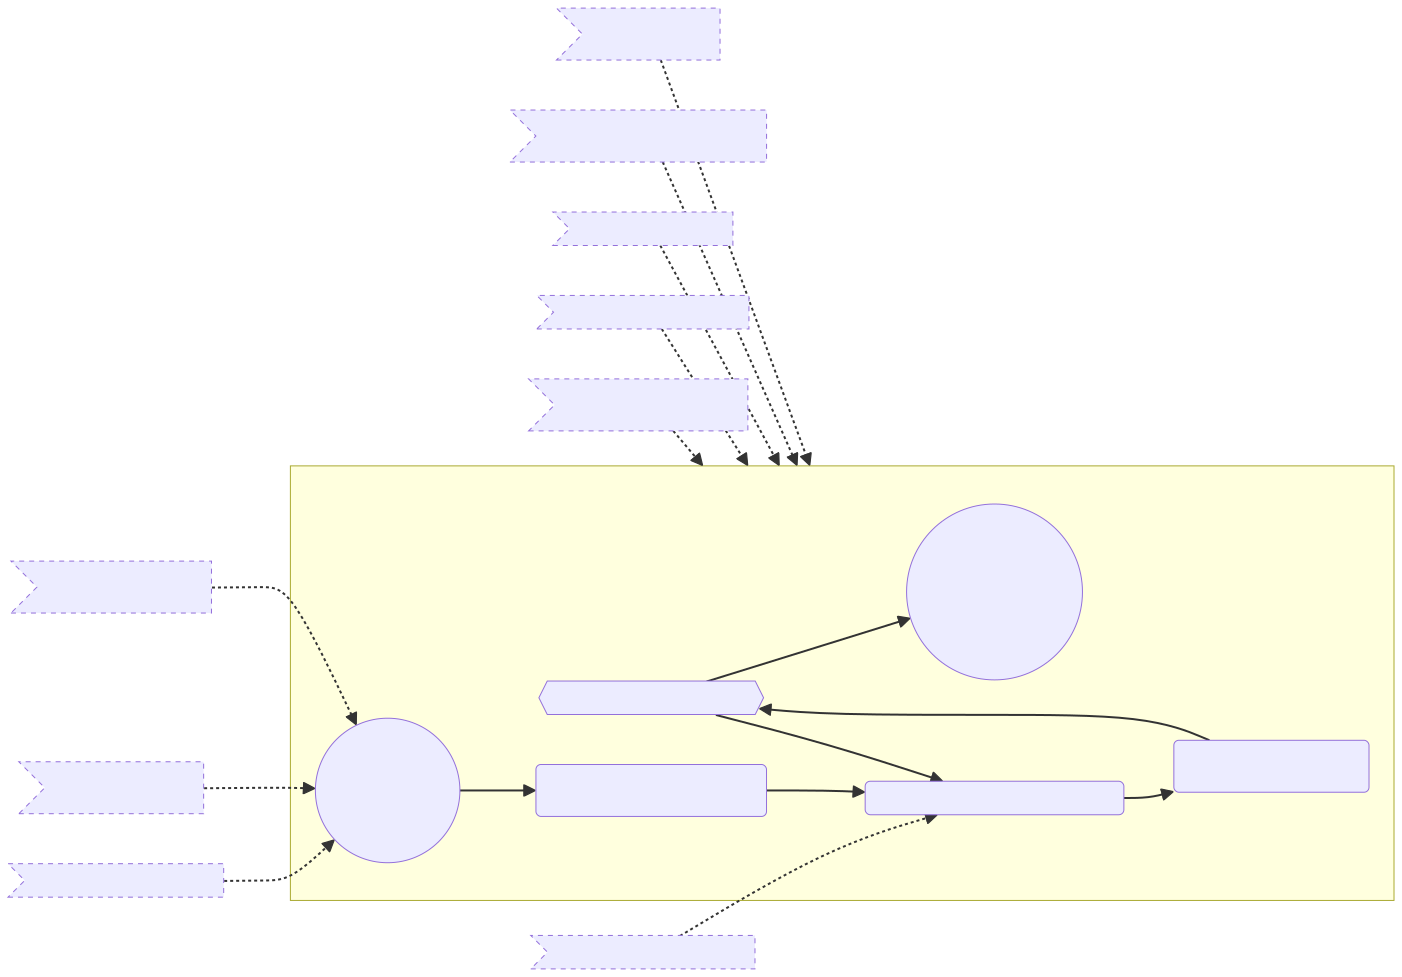
\includegraphics[width=\columnwidth]{60_optimisation_with_aspects/diagrams/aspect_applied_model.png}
  \caption{A flowchart describing a simulated game of RPGLite, and all aspects woven into the game to implement the various models of learning. Some aspects should not be woven together in the same experimental run, as they implement different models of learning.}
  \label{fig:all_aspects_applied}
\end{figure}


\subsection{Aspects for model improvement}\label{subsec:aspects_improving_model}

\subsubsection{Ensuring the Best Move is Played}\label{aspect_to_ensure_best_move}

% We make sure players always make the best moves, because it reduces the space of
% situations where randomness can skew our results. An analysis of how well this
% reflects real-world player interactions can be found in \inline{Cite William's
% thesis for realism of players making perfect moves.}


Experiments model players' character selection rather than move selection as
explained in \cref{learning_model_definition}; however, in the naive model
players randomly select moves. This is liable to place players in
unrealistically weak positions, as players are unlikely to make obviously poor
moves such as skipping a potentially useful turn. This is a concern when
modelling players learning to select characters because the learning model
relies on a causal relationship between what is observed (characters which most
reliably win games) and behavioural change (players choosing those characters).
If selecting random moves causes simulated players to lose games when they would
have won them when selecting moves realistically then move selection would
affect character selection. Realistic character selection and move selection are
therefore related.

Players of RPGLite usually selected moves optimally. In the majority of cases
\citet{kavanagh2021gameplay} found that players chose the best move available to
them: \emph{``\textelp{} the majority of actions taken were optimal, with a cost of
0.0. In total 73\% of the player's season 1 actions and 77.8\% of their season 2
actions were optimal.''}\footnote{Different seasons of RPGLite are discussed in
more depth in \cref{seasons_of_rpglite}.} Move selection can be realistically
modelled in around \(\frac{3}{4}\) of cases by selecting the best move at every
opportunity. This behaviour is implemented in an aspect by performing a lookup on
the dataset of action costs defined by \citet{kavanagh2021gameplay} and
selecting the known-optimal move in every case. This is woven into the naive
model's \lstinline{get_moves_from_table} function, which looks up moves from the
table of valid moves produced by \citet{kavanagh2021thesis}. It is invoked after
the function runs and alters its return value to include only the optimal move,
rather than all possible moves. Its source is included in
\cref{fig:best_move_aspect_source} as an example of the aspects implemented for this
thesis.\inline{Include a reference to the repo for the experiments' source code
so folk can see the other aspects too.}

\begin{figure}[h]
  \centering
  \lstinputlisting[style=custompython]{60_optimisation_with_aspects/snippets/select_best_move_aspect.py}
  \caption{An example of the implementation of an aspect for developing
  experiments around the naive model. This aspect ensures that the optimal move
  is selected by replacing the return value of \lstinline{get_moves_from_table}
  with the optimal move the function returned.}
  \label{fig:best_move_aspect_source}
\end{figure}

The aspect selecting optimal moves handles another concern of move
selection. As simulated players' behaviours are augmented to select universally
optimal moves, an anomaly in the dataset was identified. In some games, optimal
play results in infinite loops: players can arrive in a state where they would
skip turns mutually and indefinitely.

This occurs because barbarians deal more damage once they lose a sufficient
number of hit points. As a result, dealing damage to a barbarian can result in
their having an opportunity to win in one move rather than two in certain health
states. Both players can concurrently exist in this state. Therefore, both
players' optimal move is to skip their turn. \citeauthor{kavanagh2021gameplay}
note that such states were reached in 64 cases in real-world play but real-world
players never skipped their turn. To better mimic real-world play, the aspect
returns random moves if the previous two moves in a game skipped. Such a state
indicates that the game reached a state where neither player would deal damage
to the other when making optimal moves.


\subsubsection{Handle Game States with no Viable Moves}

A consequence of playing games using only optimal moves is that unexpected
states can occur: the dataset of possible moves produced by
\citet{kavanagh2021thesis} maps game states to moves a player may make, but not
all states exist in the dataset. This is because the dataset was produced
through model checking with the aim of identifying the cost of an action regards
its impact on a player's chance of winning. If a loss is guaranteed, all moves
have a 0\% chance of winning; the model checker which produced the dataset of
available moves therefore identified that the outcome of the game is already
determined in those cases, and produced no possible moves for them. 

The winning player in this situation is the player who made the previous move,
as the now-active player has no moves with a chance of winning above 0\%. This
logic is added to the model through an aspect which handles exceptions raised by
move selection, catching errors caused by an invalid table lookup. After
identifying that the exception indicates that the state does not exist (in this
case the relevant exception is Python's \lstinline{KeyError}), the aspect
handles the exception by assigning the losing player's characters 0 health and
swapping active players. The game proceeds with the losing player taking the
following turn. As this turn starts with the active (losing) player having 0
health, the game ends as expected.


\subsection{Aspects for Instrumentation}\label{subsec:aspects_instrumenting_model}

\subsubsection{Update Model of Confidence}
\label{confidence_model_aspect_impl_writeup}

As described in \cref{subsec:confidence_model}, confidence is modelled as a
Birch curve. This aspect updates a player's level of confidence using the birch
curve when a game ends. It is woven as a prelude to the naive model's
\lstinline{choose_character_pair} function, so that confidence is updated for
each player before it is used for character pair selection.

The aspect updates a value in the model's environment which represents the
confidence of the player selecting a character pair. The aspect uses the model's
environment to find parameters such as players' initial confidence or the value
of the curve's shape parameter $c$. The implementation of the aspect updating
the confidence model is given in
\cref{fig:update_confidence_model_aspect_source}. It is implementation
edited for readability, as the version used when running experiments contained
debugging code and additional logic used by abandoned experiments.

\begin{figure}[h]
  \centering
  \lstinputlisting[style=custompython]{60_optimisation_with_aspects/snippets/update_confidence_curve_aspect_edited.py}
  \caption{An example of the implementation of an aspect tracking model state.
  This aspect updates the value of a player's confidence model and is woven as
  prelude to the naive model's \lstinline{choose_character_pair} function.}
  \label{fig:update_confidence_model_aspect_source}
\end{figure}

\subsubsection{Record Prior Distribution of Character Preferences}

\inline{
  Keeping this in because I might need to explain the aspect, but it's only used
  in the implementation of choosing based on prior distribution, which I don't
  believe is ever applied. So! Decide whether to get rid of the writeup of that
  model. If I \emph{am}, then get rid of this too. If not, add it to the
  learning models writeup below and explain it here.
}
\inline{
  The above inline todo is from the summer --- things have changed a LOT since
  then! This is no longer the case, but I'm leaving the inline todo in for now
  as a reminder of the state of the writing. Can't edit at present, I'm just
  reorganising.
}




\subsubsection{Record Character Pair Choices}
It is important to keep track of the characters chosen by simulated players, as
this data is required to analyse the outcome of the experiment~\inline{Do we
describe an experiment singular or experiments plural in
\cref{chap:exp1_simulation_optimisation}?} outlined in this chapter. However,
the naive model makes no special accommodation for the collection of character
choices made by players. Character choices could be calculated by iterating
through the list of completed games after a simulation is complete, filtering
for games relating to a specific player. However, the collection of character
selection data can be simplified by tracking what was played at the end of a
game. This is achieved with with an aspect which observes the character pairs
played in a completed game, and appends each players' chosen pairs to their own
list. This aspect is applied after its join point executes (an ``encore'' in
PyDySoFu parlance\inline{reference pdsf's explanatory chapter / re-engineering
chapter here? unsure which is most appropriate / introduces the concepts
first.}).

There are many ways to collect this data, aspectually or otherwise; however, the
simplicity of collecting information mid-process without requiring modification
of a base model demonstrates the flexibility of an aspectual augmentation of
models and simulations as an approach. Collection of chosen character pairs
mid-simulation is an opportune example of this convenience.

\subsubsection{Track Detailed Outcomes of
Games}\label{subsubsec:detailed_game_outcome_tracking_aspect} Similarly to the
recording of character pair choices, the outcomes of games must be tracked. This
information is important as an input of our model of learning, as successes and
failures observed by players for each character pair can inform their models of
learning. Some models of learning implemented, such as one including a
hyperbolic decay bias (to be explained later, in
\cref{subsubsec:learning_with_hyperbolic_decay}), require not only knowledge of
the proportion of wins each character pair has achieved, but also the history of
wins and losses: players might be biased toward recent win/loss observations,
discounting older experiences in favour of the new. Detailed historical win/loss
information must therefore be recorded.

As with character pair choices, the naive model was not engineered with the
intention of providing this information specifically. However, the model is
easily instrumented to collect such information at many suitable points. As with
recording a player's chosen character pairs, an ``encore'' aspect was
implemented which records wins and losses observed for character pairs on game
end. Specifically, the aspect models players observing character pairs which won
at the end of a game, lost at the end of a game, and also pairs which were
uninvolved in the game. This requires a list of outcomes (wins, losses, and
neither) for every player, for every character pair. The lists of observed
outcomes for a given character pair record \lstinline{True} for a winning pair,
\lstinline{False} for a losing pair, and \lstinline{None} for a character which
was not involved in the game's outcome. Each player observes the relevant state
for every character at the end of any game they play. Provisions were made in
the implementation of this aspect for a player only paying attention to their
own outcomes (i.e. only recording whether their own pair won or lost, without
consideration for their opponent's outcome), though in practice all simulations
were performed with players observing both their own outcomes and those of their
opponents.

\subsubsection{Record Winning Pair observed by Players on Game
End}\label{subsubsec:aspect_to_observe_winning_pair} Unlike the detailed game
outcome data recorded by the aspect described in
\cref{subsubsec:detailed_game_outcome_tracking_aspect} and used in advanced
learning models such as that of hyperbolic decay (to be explained later, in
\cref{subsubsec:learning_with_hyperbolic_decay}), other learning models required
only simple outcome data. The simpler model of learning making use of a
distribution of winning teams to be explained in
\cref{subsubsec:learning_by_picking_from_distribution_of_wins_with_confidence}
is more easily implemented against a simple list of winning teams. Rather than
coalescing the more complex dataset collected as described in
\cref{subsubsec:detailed_game_outcome_tracking_aspect} to achieve the desired
format, another aspect can be applied to collect the data in a simpler format
directly.

An aspect was implemented which also models players observing winning character
pairs on game end, but collects the data in a simple list of character pairs
observed to win games, rather than a mapping of character pairs to game end
states as described in \cref{subsubsec:detailed_game_outcome_tracking_aspect}.
Character pairs which lose games or are not involved are not recorded for the
purpose of the alternative model of learning.

% TODO: Section / subsection for models of learning
\subsection{Aspects Implementing Models of Learning}\label{subsec:aspects_modelling_learning}

% * The aspects already described explain how we set up the model for applying our learning implementations,
%   both instrumenting it for observation and tweaking fundamental behaviours.
% * Now we need to implement models of learning! We'll present two.
% * First, a simple model of learning as described in \cref{subsec:models_of_learning_discussed}
%   which uses a confidence sigmoid to discern between selecting character pairs based on what was 
%   previously observed to win games, and random selections representing exploration of a player's options.
% * Second, a more complex model of learning which applies the same concepts, but introduces a hyperbolic decay
%   on the simulated player's learning, introducing a biased model of learning.

\inline{Still editing but the other two subsections have no intro; right now this has three paras!}

The aspects described above implement setup for the models of learning applied
in this thesis, both instrumenting the underlying RPGLite model for observation
and tweaking behaviours of the naive model. Two aspects remain unexplained,
implementing the learning models themselves.

The first model of learning left to be described is implemented as described in
\cref{subsec:models_of_learning_discussed}, drawing from a record of character
pairs observed to win in earlier games to select characters in future games, in
accordance with a model of confidence which activates either this behaviour or a
randomly selected pair. A detailed description follows in
\cref{subsubsec:learning_by_picking_from_distribution_of_wins_with_confidence}.

The second model of learning left to be described implements a similar logic,
but introduces a weighting on the history of winning pairs a player observes,
introducing a hyperbolic discounting bias to historical observations. In this
model, players increasingly discount old observations in favour of recent ones.
A model of learning with a hyperbolic discounting bias is described in
\cref{sec:optimisation_with_aspects_experimental_design}.

% \subsubsection{Character Selection from prior distribution}
% ==== NOTE: the above subsubsection references an aspect where characters are picked directly from
%            the prior distribution from a training set, and doesn't contain a model of learning at all.

\subsubsection{Character Selection using Prior Distribution}

\inline{
  WRITE ME
  WRITE ME
  WRITE ME
  WRITE ME
  WRITE ME

  Need to define the model which selects characters using the prior distribution.
}

\subsubsection{Character Selection using confidence sigmoid}\label{subsubsec:learning_by_picking_from_distribution_of_wins_with_confidence}

The first model of learning applied through aspect orientation draws on
character pairs a simulated player observed to have won games (as recorded by
the relevant instrumenting aspect, discussed in
\cref{subsubsec:aspect_to_observe_winning_pair}). The record of previously
winning character pairs defines a probability mass function by selecting a
character with equal probability to their rate of appearance in the history of
winning characters.

Selecting a character based on this distribution is gated by a confidence model
as described in \cref{subsec:confidence_model}. If a simulated player's
confidence model indicates insufficient experience to found decisions on,
players will instead select characters randomly, effectively exploring their
space of possible choices. By doing so, players have the time and opportunity to
observe many matchups between different character pairs. Time to observe
matchups is important because some character pairs may only present a strong
choice if played against specific alternatives. We can imagine a character pair
which is extremely effective against 50\% of pairs, but extremely likely to lose
games played against the remaining 50\% of possible opponents. Without exploring
possible matchups, a player may lack observations which would inform them about
whether a character pair is effective in general, or in a narrow set of
circumstances. A confidence model encouraging early exploration promotes the
experience of a wide variety of matchups, avoiding this issue.

Another concern early exploration mitigates is that simulated players need
opportunities to build well-rounded priors: if a character pair is never
selected by any player, experienced players basing their character pair choices
on those which previously win games cannot include pairs which were never
selected, because they will never have had the opportunity to win games at all.

This aspect was implemented as an ``around'' aspect in PyDySoFu's parlance,
allowing it to apply additional logic before and after its join point. It could
equally appropriately have been implemented as an ``encore'', applying logic
only after its join point had executed; the aspect discards the random selection
made by the base model unless the simulated player lacks confidence. Either
implementation can return a different character pair choice to the join point's
caller, allowing the chosen character pair to effectively be overridden, and so
allowing the aspect-applied RPGLite model to proceed executing as it would
otherwise; the only difference being the pair of characters ``chosen'' by the
simulated player whose behaviour was augmented.


% \subsubsection{Character Selection exhibiting hyperbolic decay}\label{subsubsec:learning_with_hyperbolic_decay}

% \inline{
%   I believe I'm scrapping the hyperbolic decay model altogether. Doesn't make
%   sense to keep it given my testing \& evaluation harness right now, but I can
%   refer to it to compare the implementation (and performance…?) of around-based
%   and within-based fuzzers. Can't remove / edit now, I'm reorganising; to
%   revisit.
% }
% Character selection with hyperbolic decay works similarly to the simple model of
% learning as described in
% \cref{subsubsec:learning_by_picking_from_distribution_of_wins_with_confidence}.
% Character pairs are selected randomly if a player lacks confidence or, if the
% confidence model applied to the player indicates that character pairs are to be
% chosen according to their historical observations of winning pairs, their record
% of winning pairs in previous games informs their choices instead. However, this
% model also applies a hyperbolic discounting bias which weights the player's
% historical observations when making choices.

% Hyperbolic discounting is a bias studied in behavioural economics.
% \inline{Find citations explaining hyperbolic discounting}

% A hyperbolically discounted score for an event after a delay \(D\) with
% discounting factor \(k\) is calculated by:

% \begin{figure}
% \[score(D) = \frac{1}{1 + kD}\]
% \caption{Hyperbolic discounting score calculation}
% \end{figure}

% This score can be applied to a history of games played with different character
% pairs to weight that history; this weighting can then be used to create a new
% PMF to draw character pair choices from, by allocating each pair a probability
% of being chosen according to its share of the weighted history of winning pairs.
% Where the previous method for selecting character pairs selected each pair with
% the frequency they appear in the record of winning pairs, this method weights
% the record of winning pairs; the sum weighted history of a character pair's wins
% as a proportion of the total weighted history for all pairs becomes the PMF for
% character pair selection. \inline{Maybe there's need here for a diagram or some
% extra equations to make this clearer\ldots{}?}

% With this scoring mechanism, our model of learning incorporates a behavioural
% bias which some real-world players may exhibit. Player character choices can now
% be modelled through different behavioural variations applied to the naive model.
% The resulting behaviours from each model of learning can be compared to that
% exhibited by the naive model to discern which produces simulated RPGLite play
% more similar to a given real-world player's; methods for doing so are explored
% in the remainder of this chapter. 




\section{Experimental Design}
\label{sec:optimisation_with_aspects_experimental_design}

The models of learning described in \cref{subsec:aspects_modelling_learning} can
be applied to augment the naive model described in
\cref{sec:optimisation_with_aspects_naivemodel} and introduce change in player
behaviour over time. The remaining challenge is to demonstrate that augmenting
the naive model can make it more realistic in practice. To that end, the
remainder of this chapter details an experiment which compares synthetic
datasets produced by the model to empirically sourced data, and shows that this
synthetic data is more similar to its empirical counterpart than that produced
by a naive model with no aspects applied.\inline{Some reference to the research
question is required here.}

This section presents classes used in the design and implementation of
experiments, as they constitute the foundation of the execution and evaluation
of synthetic datasets. This is followed by documentation of the strategy for
generating synthetic datasets, and a description of the technique used to
compare them to select optimal parameters for player simulation. This design is
used in the experiment itself, described later in
\cref{sec:optimisation_with_aspects_experimental_results}.


\subsection{Optimising the Model to Simulate a Real-World Player}
\label{exp1:optimisation_strategy}

\inline{I need to write up the strat for using k-fold validation.
Should include the parameters selected, evaluation of ``best'' result, etc.}

%% OLD NOTES FROM WHEN THIS LIVED TOWARD THE END
%% TODO: DECIDE WHETHER I CAN NUKE THEM (CURRENTLY ON TUBE, DIFFICULT TO EVALUATE)

\inline{Discussion required here around the mitigation of randomness --- it's
required because of RPGLite's inherent RNG --- and also explaining how we make
use of a grid search in combination with k-fold validation to anneal toward
well-fitted parameters of our models of learning for each individual player.}

\inline{TODO make a diagram of this.}

% To mention here:
% \begin{itemize}
%   \item Data generation specifically: \begin{itemize}
%     \item Boredom. We rotate players to make sure we've got a constant stream of
%     new players being introduced into the game, and to maximise the number of
%     times a simulated player is able to explore the state space.
%     \item Data generation
%     \item normalisation.
%     \item Calculation of preference distribution lists
%   \end{itemize}
%   \item Actual annealing: \begin{itemize}
%   \item Identify the different parameters to fit, and briefly explain them and
%   their significance to the model.
%   \item Testing combinations of different parameters. Compare grid search on RGR
%   to current combine-lots-of-parameters technique.
%   \end{itemize}
% \end{itemize}





\subsection{Model parameters}
\label{subsec:exp1_model_parameters}

Many parameters are used to control simulated play of RPGLite. Their use in
modelling learning or running simulations for data generation is explained in
following subsections; however, parameters which control an experimental run are
collected in a class, \lstinline{ModelParameters}. Defining these values in a
class helps to identify them in the codebase, and defines all variables which
are used when optimising the model.\inline{These parameters are required because
we run with different parameters for different folds. This subsec should be
preceded by another on our strategy for optimising, so we can introduce k-fold
validation and clean up the wording in this sec so it makes more sense.}

\begin{figure}
  \begin{center}
    \begin{lstlisting}
from dataclasses import dataclass

@dataclass
class ModelParameters:
    c: float
    curve_inflection_relative_to_numgames: float
    prob_bored: float
    boredom_enabled: bool
    training_data: list
    testing_data: list
    assumed_confidence_plateau: float
    starting_confidence: float
    iteration_base: int
    number_simulated_players: int
    advice: list[tuple[str, str, str|callable]]
    players:list[str]
    args:list[any]
    kwargs:dict[str:any]
    boredom_period: int = 25
    initial_exploration: int = 28

    @property
    def boredom_period(self) -> int:
        '''
        Number of games to play before checking player boredom.
        Attempts to allow every player combo to play each other once on average before checking again.
        '''
        return int(self.number_simulated_players**2)/2

    def active_dataset(self, testing) -> list:
        return self.testing_data if testing else self.training_data

    def iterations(self, testing) -> int:
        '''
        The number of games to play when generating a synthetic dataset
        '''
        if self.boredom_enabled:
            return self.iteration_base
        return int(self.number_simulated_players**2 * len(self.active_dataset(testing)) / 2)

    def rgr(self, testing) -> float:
        '''
        RGR for the parameterised c value, number of games to play, and start/end confidences.
        '''
        if not hasattr(self, '_rgr_cache'):
            self._rgr_cache = dict()
        if self._rgr_cache.get(testing) is None:
            num_games_to_confidence = len(self.active_dataset(testing)) * self.curve_inflection_relative_to_numgames
            self._rgr_cache[testing] = \
                curveutils.rgr_yielding_num_games_for_c(
                    num_games_to_confidence,
                    self.c,
                    start=self.starting_confidence,
                    limit=self.assumed_confidence_plateau)
        return self._rgr_cache[testing]
    \end{lstlisting}
  \end{center}
  \caption{A class defining the parameters of the model of learning RPGLite which vary when optimising for a given player. For layout \& space reasons, some methods of minor significance are removed.}
  \label{fig:model_parameters_class}
\end{figure}

The \lstinline{ModelParameters} class is shown in
\cref{fig:model_parameters_class}. The parameters it defines, briefly explained,
are:\label{list_of_model_parameter_attributes}\inline{IIRC Tim doesn't love the description list formatting. Probably
means I should avoid; consider other ways of laying this out that avoids a big
wall of text}

\begin{description}
  \item[starting\_confidence] The initial value of the model's confidence curve.
  \item[assumed\_confidence\_plateau] A corresponding high value for the model's
  confidence curve. As the curve's growth rate is calculated to align with the
  number of games completed by the real-world player being simulated, and the
  curve asymptotically approaches 1, a high value is required which represents
  the expected confidence of a real-world player having played a significant
  number of games.
  \item[curve\_inflection\_relative\_to\_numgames] The proportion of games played by
  the real-world player being simulated at which the player's confidence
  curve should reach the parameter \lstinline{assumed_confidence_plateau}. This
  allows for control over the growth rate of the curve while linking the rate of
  growth to the number of games played by the real-world player being simulated;
  \item[C] The curve parameter of the confidence model's underlying birch curve;
  \item[prob\_bored] The probability that a player with confidence above
  \lstinline{assumed_confidence_plateau} becomes ``bored'' and stops playing
  RPGLite. These players are removed from the simulated playerbase and replaced
  with new players. This mechanism is discussed in further detail in
  \cref{subsec:controlling_state_space_exploration}.
  \item[boredom\_enabled] Whether the boredom mechanism discussed in
  \cref{subsec:controlling_state_space_exploration} is to be enabled.
  \item[training\_data] The set of real-world games used as a training fold when
  optimising parameters for simulating a player.
  \item[testing\_data] The set of real-world games used as a testing fold when
  optimising parameters for simulating a player.
  \item[iteration\_base] The number of games to play when generating a synthetic
  dataset. If \lstinline{boredom_enabled==False}, the number of games is instead
  calculated to ensure that all synthetic players play the same number of games
  as were completed by the played being simulated, (calculated from the training
  or testing fold as appropriate).
  \item[number\_simulated\_players] The size of the simulated playerbase.
  \item[advice] A list of tuples defining advice to weave when generating data.
  Pieces of advice are uniquely defined by a tuple containing the type of aspect
  to weave (such as \lstinline{"prelude"} or \lstinline{"error_handler"}), a
  string-represented regular expression defining the join point of the advice,
  and a \lstinline{callable} to use as an aspect when weaving the advice. As
  \lstinline{ModelParameters} instances are serialised to disk to persist
  experiment results and Python functions are not seralisable, this may also be
  a string value; strings are IDs of aspects, and are replaced with their
  corresponding aspect on deserialisation.
  \item[players] The player being simulated. This parameter is a list of player
  usernames to support simulating groups of players if required, though this
  functionality is not used in the experiments presented in
  \cref{chap:experimental_results}.
  \item[args] Any additional arguments to pass when running a simulation.
  \item[kwargs] Any additional keyword arguments to pass when running a simulation.
  \item[boredom\_period] The number of games completed by the simulated
  playerbase between checks of players' confidence and random selection for
  removal (default 25).
  \item[initial\_exploration] A value which controls the number of
  games individual players complete before their confidence \& learning models control
  their character pair selection (default 28, to allow sufficient games to
  select every available pair exactly once).
\end{description}

\begin{figure}
  \begin{center}
    \begin{lstlisting}
class ModelParameters:

    # <snipped additional attributes and methods for space>

    def run_experiment(self, testing, correlation_metric):
        real, synthetic = generate_charpair_distributions(\
            rgr_control=self.rgr(testing=False),
            iterations=self.iterations(testing=False),
            games=self.training_data,
            players=self.players,
            birch_c=self.c,
            sigmoid_initial_confidence=self.starting_confidence,
            boredom_confidence=self.assumed_confidence_plateau,
            num_synthetic_players=self.number_simulated_players,
            boredom_period=self.boredom_period,
            prob_bored=self.prob_bored,
            advice=self.advice,
            *self.args,
            **self.kwargs)
        return Result(self, real, synthetic, correlation_metric, testing)
    \end{lstlisting}
  \end{center}
  \caption{The \lstinline{run_experiment()} method on the
  \lstinline{ModelParameters} class, which can be used to reproduce an
  experimental run from its parameters.}
  \label{fig:ModelParameters_run_experiment_method}
\end{figure}

These parameters are varied when optimising the model to represent the learning
of individual players in order to find a combination of parameters which best
represent a given player.\footnote{The strategy for this optimisation is
described in \cref{exp1:optimisation_strategy}.} A \lstinline{ModelParameters} object defines
everything required to run a simulation of RPGLite play and produce the
resulting character pair distribution for analysis. 
Individual experimental runs\footnote{Throughout this chapter, ``experimental run''
is used to refer to the process of producing a simulated dataset for comparison
against training or testing folds taken from the dataset of completed RPGLite
games. Many experimental runs with different parameters are used to optimise a
model.} can therefore be reproduced using the class. 
The convenience method \lstinline{run_experiment()}, as shown in
\cref{fig:ModelParameters_run_experiment_method}, is provided to simplify
reproducing experimental runs with \lstinline{ModelParameters} objects.


\subsection{Representing the result of an experimental run}

As referenced in \cref{fig:ModelParameters_run_experiment_method}, a
\lstinline{Result} class is defined to collect the results of an experimental
run and simplify analysis of the distribution of character pair selection
produced. A definition of the \lstinline{Result} class is given in
\cref{fig:Result_class}. This class is used in the analysis of the success of an
experimental run when selecting ideal experimental parameters for the simulation
of a real-world player.

A \lstinline{Result} is not the result of an entire experiment, or the ideal
parameters to simulate a given player. Instead, it represents the result of
attempting to generate realistic data for a player, which is defined by a
\lstinline{ModelParameters} attribute. Several \lstinline{Result} objects can be
compared against desired probabilities of correlation and correlation statistics
(the \lstinline{pval} and \lstinline{statistic} properties, respectively) to
select an optimal set of parameters for the simulation of an RPGLite player.


\begin{figure}
  \begin{center}
    \begin{lstlisting}
from dataclasses import dataclass
@dataclass
class Result:
    params:ModelParameters
    real_distribution:list[float]
    simulated_distribution:list[float]
    correlation_metric:Optional[callable]
    testing: bool

    @property
    def pval(self) -> float:
        return self.correlation_metric(self.real_distribution, self.simulated_distribution).pvalue

    @property
    def statistic(self) -> float:
        return self.correlation_metric(self.real_distribution, self.simulated_distribution).statistic

    def within_acceptable_bounds(self, pval_threshold:float, statistic_threshold:float) -> bool:
        return self.pval < pval_threshold and self.statistic > statistic_threshold
    \end{lstlisting}
  \end{center}
  \caption{The \lstinline{Result} class used to collect results of experimental
  runs and evaluate their success.}
  \label{fig:Result_class}
\end{figure}


\subsection{Quantifying Similarity of Character Pair Selection}
\label{measuring_charpair_similarity}

\inline{This subsection most likely needs to be condensed.}
The experiments presented in this chapter make comparisons of many synthetic
datasets against a single empirically sourced dataset. The latter contains all games
completed by a player whose learning of RPGLite we aim to simulate, and is drawn
from the published RPGLite dataset~\cite{rpglite_dataset}. Comparisons are
required to determine which of the synthetic datasets most closely matches the
empirical dataset. We are specifically interested in determining whether players
played with preference toward similar character pairs. The distribution of their
choices describes a bias toward some pairs, and away from others. The
distribution of the naive model, being randomly chosen, should exhibit no bias;
a simple null hypothesis is therefore that a simulated dataset is as similar to
real-world play as a randomly generated one; there exists no bias comparable to
that exhibited by the empirical dataset in this case. Our hypothesis in
answering the first research question posed is that, with models of learning
applied through aspect orientation, the naive model can exhibit biases toward
character pairs similar to that of a real-world dataset. The simulated play
would therefore exhibit a more ``realistic'' behaviour in character selection
than the naive model as a result of the aspects applied.

We expect discrepancies in the specific character pairs selected in games (such
as the order of character selection) because of the random nature of character
selection. However, it is feasible to assess the similarity between the
distribution of character pairs chosen by simulated and real-world players. The
distribution of a player's chosen character pairs describes the preferences of
that player, as it allows their selections to be ranked. We can examine the
similarities between a player's character pair preferences and the preferences
of simulated players by ranking and correlating their preferences to arrive at a
measurement of similarity between the datasets; this is achieved through
rank correlation.

Many rank correlation measurements exist. For the purpose of comparing lists of
character pairs, we require a non-parametric measurement. Some methods for
calculating correlation assume a distribution of data, or require data to be
distributed in a consistent manner; as nothing is known about the distribution
of character choice preferences (and this distribution could vary between
players), a measurement which is independent of the underlying distribution is
required. Two common options are Spearman's \rho and Kendall's \tau.
\inline{Find citations for each correlation coefficient, and also for justifying choosing between these two specifically (if required).}
These measurements assess correlation in different ways, which can affect
measurements of character pair preference. Spearman's \rho accounts for the
magnitude of difference between ranks, and is calculated as $\rho = 1 - \frac{6
\sum (d^{2}_{i}}{n(n^{2}-1)}$, where $d^{2}_{i}$ is the difference in the rank
of the $i^{th}$ observation in each dataset and $n$ is the total number of
datapoints in a dataset. Kendall's \tau{} accounts only for their ordering. It
can be calculated as $\tau = \frac{C - D}{C + D}$, where $C$ is the count of
concordant pairs, and $D$ the count of discordant pairs.

To choose an appropriate measure, we relate them to potential patterns in our
datasets. As we expect many character pairs to be infrequently picked (if at
all) once players develop preferences, a slight increase in selecting uncommon
character pairs within a simulation could incur a significant increase in rank.
This would have a more significant impact on \rho{} than on \tau{}, as the
larger difference in rank is squared in the calculation. The simulated dataset
might also produce a distribution where rankings between empirically sourced and
synthetic datasets had small differences, but were similarly positioned
throughout the dataset. This would have an outsized impact on \tau{}, as
relative positioning affects concordance, but the square of a small difference
in rank remains relatively small, meaning that \rho{} would be less affected by
this pattern. A choice of correlation metric is thus a choice of what
correlation means: should correlation more closely reflect preference of
character pairs relative to each other, or ``forgive'' small relative preference
deviations but impose a greater cost on the scale of disagreement on a given
rank?

We choose to prioritise the preservation of rank order~(\tau{}) over the
minimisation of rank difference~(\rho{}). Unfavoured character pairs' ranks
might be affected greatly by a small difference in the number of games played,
because unfavoured character pairs play few games by definition. A small
difference in selection count is therefore more likely affect rank; however, the
character pairs would still be unfavoured relative to a players' preferred
pairs, which are expected to have a disproportionately high number of games,
also by definition. Minimising rank difference is therefore sensitive to
RPGLite's random nature. Preserving the ordering of character pair selection is
also important when considering favoured pairs, as differences might indicate a
difference in patterns of play; however, small differences in the ranks of
favoured pairs with \rho{} would have a less signifiant impact than when
measuring rank ordering with \tau{}: \rho{} accounts for the square of the
difference in rank, which remains small for small differences.

For these reasons, we quantify similar character pair preferences by
representing preference as an ordered list of string-represented character
pairs, and measuring their correlation using \tau{}. \inline{I'm not sure I've
  defined how I represent (or calculate) the ordered list of preferences yet. If
  not, that should live somewhere, I suppose.}



\subsection{Controlling State Space Exploration}
\label{subsec:controlling_state_space_exploration}

The model of confidence used grows monotonically as described in
\cref{subsec:defining_our_models_of_learning}, which affects simulated players'
exploration of possible character pairs. Models of learning use confidence as a
probability that their alternative behaviour is to be encoded; therefore, when
confidence is high, players are likely to select character pairs to play which
were observed to be likely to win historically. As character pairs which are not
played cannot win games, pairs which are not selected for play cannot be chosen
by models of learning which rely on a players' historical observations, which
could lead to inaccurate simulation. To counter this possibility, two mechanisms
are introduced to control state space exploration: ``initial exploration'' and
``boredom''.

\inline{A little clumsy --- reword this para? Is it sufficent? } Initial
exploration is a threshold number of games a simulated player must complete
before models of learning make changes. Learning models' impact in player
behaviour is gated on both a player's level of confidence and the number of
games played. This allows players to observe enough win/loss data in their early
games that later decisions directed by the learning model have sufficient
historical observations to have explored the state space make ``informed''
decisions. The length of the initial exploration phase for any player is given
as an integer number of games by the \lstinline{initial_exploration} parameter
when generating data, as mentioned in \cref{subsec:exp1_model_parameters}; use
of the parameter when generating data is discussed in
\cref{subsec:exp1_producing_datasets}.

Boredom is a mechanism which solves a problem introduced by some combinations of
model parameters: if the confidence model's growth rate and curve parameter are
high, player confidence raises sharply, with the effect that simulated players
are unlikely to explore the state space. A situation can arise where the
simulation's metagame\revnote{At time of writing metagame is not defined, but
this should be introduced in \cref{chap:rpglite}; there's a corresponding
revision note there.} falls into a local optimum, where the entire playerbase
collectively observe many historical wins for some character pairs because of a
disproportionately high rate of random selection when players explore the space
of possible character pairs. This can be overcome by introducing new players
into the playerbase over time. New players are guaranteed to explore the state
space due to the initial exploration phase, and will continue to do so while
their confidence grows. The randomly selected character pairs played in this
time means veteran players will play games which would not be selected
otherwise. This reinforces existing preferences when novel character pairs are
weaker than veteran players' preferences, and weakens existing preferences if
veteran players are exposed to novel character pairs which are likely to win
games played against their preferred pairs. In disrupting a locally-optimal
search of the space of character pairs, boredom mitigates potential issues with
random play, while allowing simulated players to learn over time.

Boredom is implemented using several parameters. Players are eligible to be
removed from the playerbase when their model of confidence reaches a threshold,
defined by \lstinline{assumed_confidence_plateau} as mentioned in
\cref{subsec:exp1_model_parameters}. Once this threshold is reached, each player
is removed with probability \lstinline{prob_bored}, allowing some confident
players to remain in the playerbase for a long time. \inline{TODO note that
players are removed, and then replaced, so that the playerbase is of constant
size but varying experience! Replacement happens immediately.}\inline{Mention
boredom period controlling how often we check that players are bored.}\inline{TODO note that
boredom can be disabled}




\subsection{Producing Datasets}\label{subsec:exp1_producing_datasets}

% A brief explanation of `generate_synthetic_data`, to separate it from the
% annealing below.
% It's responsible for:
% - Setting up special vals consumed by aspects in the games' environment dict
% - weaving aspects (and un-weaving them)
% - matching players together and kicking off games
% - Recycling players when they get ``bored''

Our goal is to produce datasets of simulated player behaviour with aspects
applied. This is achieved by weaving aspects to augment behaviour and repeatedly
invoking the naive model's \lstinline{play_game} function while managing the
simulated playerbase.\footnote{For example, generating synthetic datasets
  involves } The experimental codebase contains
a function which is responsible for these tasks,
\lstinline{generate_synthetic_data}, which is parameterised as follows:
\revnote{I end list items here with semicolons. I should be consistent through
  the thesis, and decide whether semicolons are appropriate.}

\begin{itemize}
  \item \lstinline{rgr_control:float}, which is the RGR value provided by the
  \lstinline{rgr(testing:bool) -> float} method of a \lstinline{ModelParameters}
  instance. This is passed to \lstinline{generate_synthetic_data} directly
  to maintain ignorance within the function as to whether it is training or
  testing against a dataset; the caller is aware instead, and passes the correct
  RGR value;
  \item \lstinline{environment:dict()}, the environment simulated players interact
  with, which is used to accumulate information shared by all players such as a
  history of games or special values used to parameterise aspect behaviour;
  \item \lstinline{params:ModelParameters}, the \lstinline{ModelParameters}
  instance which provides parameters detailed in
  \cref{list_of_model_parameter_attributes} and is used to parameterise aspect
  behaviour and the model of boredom used to manage players;
  \item \lstinline{print_progress:bool=False}, a parameter controlling the
  printing of debug loglines.
\end{itemize}

This is sufficient to generate a synthetic dataset, as all values which
parameterise the behaviour of simulated players are encapsulated in the
\lstinline{ModelParameters} class. 



% Weaving aspects, unweaving at the end
% creating and matching synthetic players
% Model of boredom (which can be switched off, importantly)


\subsection{Answering the first Research Question}
\inline{
  THIS SHOULD BE MOVED TO THE NEXT CHAPTER. There are lots of issues here. We're
  answering the second RQ now, not the first; also, we need to introduce the
  results of the prior distribution model before talking about answering the RQs.
}
In designing advice which amends a model with new behaviour, the first research
question was effectively answered:

\begin{researchquestion}
  Can changes to a model be represented as advice using aspect orientation?
\end{researchquestion}

The advice described in this chapter demonstrates that behavioural variations
such as learning can be separated into aspects and applied to a model to alter
its behaviour without requiring its original implementation to be modified. We
can therefore answer this research question: \emph{yes}, modifications to a
model can be represented using advice.

\inline{A note here that we're using AOP, but don't actually target
  cross-cutting concerns in our models of learning, which is interesting.}

\inline{This is no longer the case; this section needs rewriting!}
Other research questions motivated in the literature review in
\cref{chap:lit_review} are concerned with whether representing changes to models
using aspect orientation can accurately reflect their subject, and whether the
modules formed by a library of aspects can be reused. These are investigated in
\cref{sec:optimisation_with_aspects_experimental_results} and
\cref{chap:exp2_old_aspects_new_systems} respectively.



\section{Discussion}
\label{sec:optimisation_with_aspects_discussion}

A closing discussion on what we found, and how the research question was
answered.

Also, note the weaknesses of the approach.

\begin{itemize}
  \item More games could have lead to a more accurate result
  \item It'd be interesting to use the models to ``learn'' other things too,
    such as move selection / mistakes made
  \item Would like to reproduce across multiple different systems, not just
    RPGLite. Maybe developers like we did in the CAISE paper, maybe aspects that
    aren't learning like degraded modes. Could be interesting to model a complex
    adaptive system with aspects representing rule changes. Could be interesting
    to demonstrate other uses of aspectually augmented systems, like introducing
    new rules to a cellular automaton.
\end{itemize}
